\section{Основные понятия и определения}

Номинальный размер(D0) --- размер, относительно которого определяются отклонения.

Предельные размеры(d + ES, d + EI) --- два предельно допустимых размера, между которыми должны находиться или которым может быть равен действительный размер годной детали.

Предельные отклонения(ES, EI) --- разность между предельным отклонением и номинальным размером.

Допуск $T$ --- разность между наибольшим и наименьшим предельными размерами или алгебраическая разность между верхним и нижним отклонениями.

Посадка --- характер соединения двух деталей, определяемый разностью их размеров до сборки.

Зазор(S) ---  разность размеров отверстия и вала, если размер отверстия больше размера вала.

Натяг(N) --- разность размеров вала и отверстия до сборки, если размер вала больше размера отверстия.

Переходная посадка --- могут получаться как зазоры, так и натяги.

\begin{figure}
	\centering
	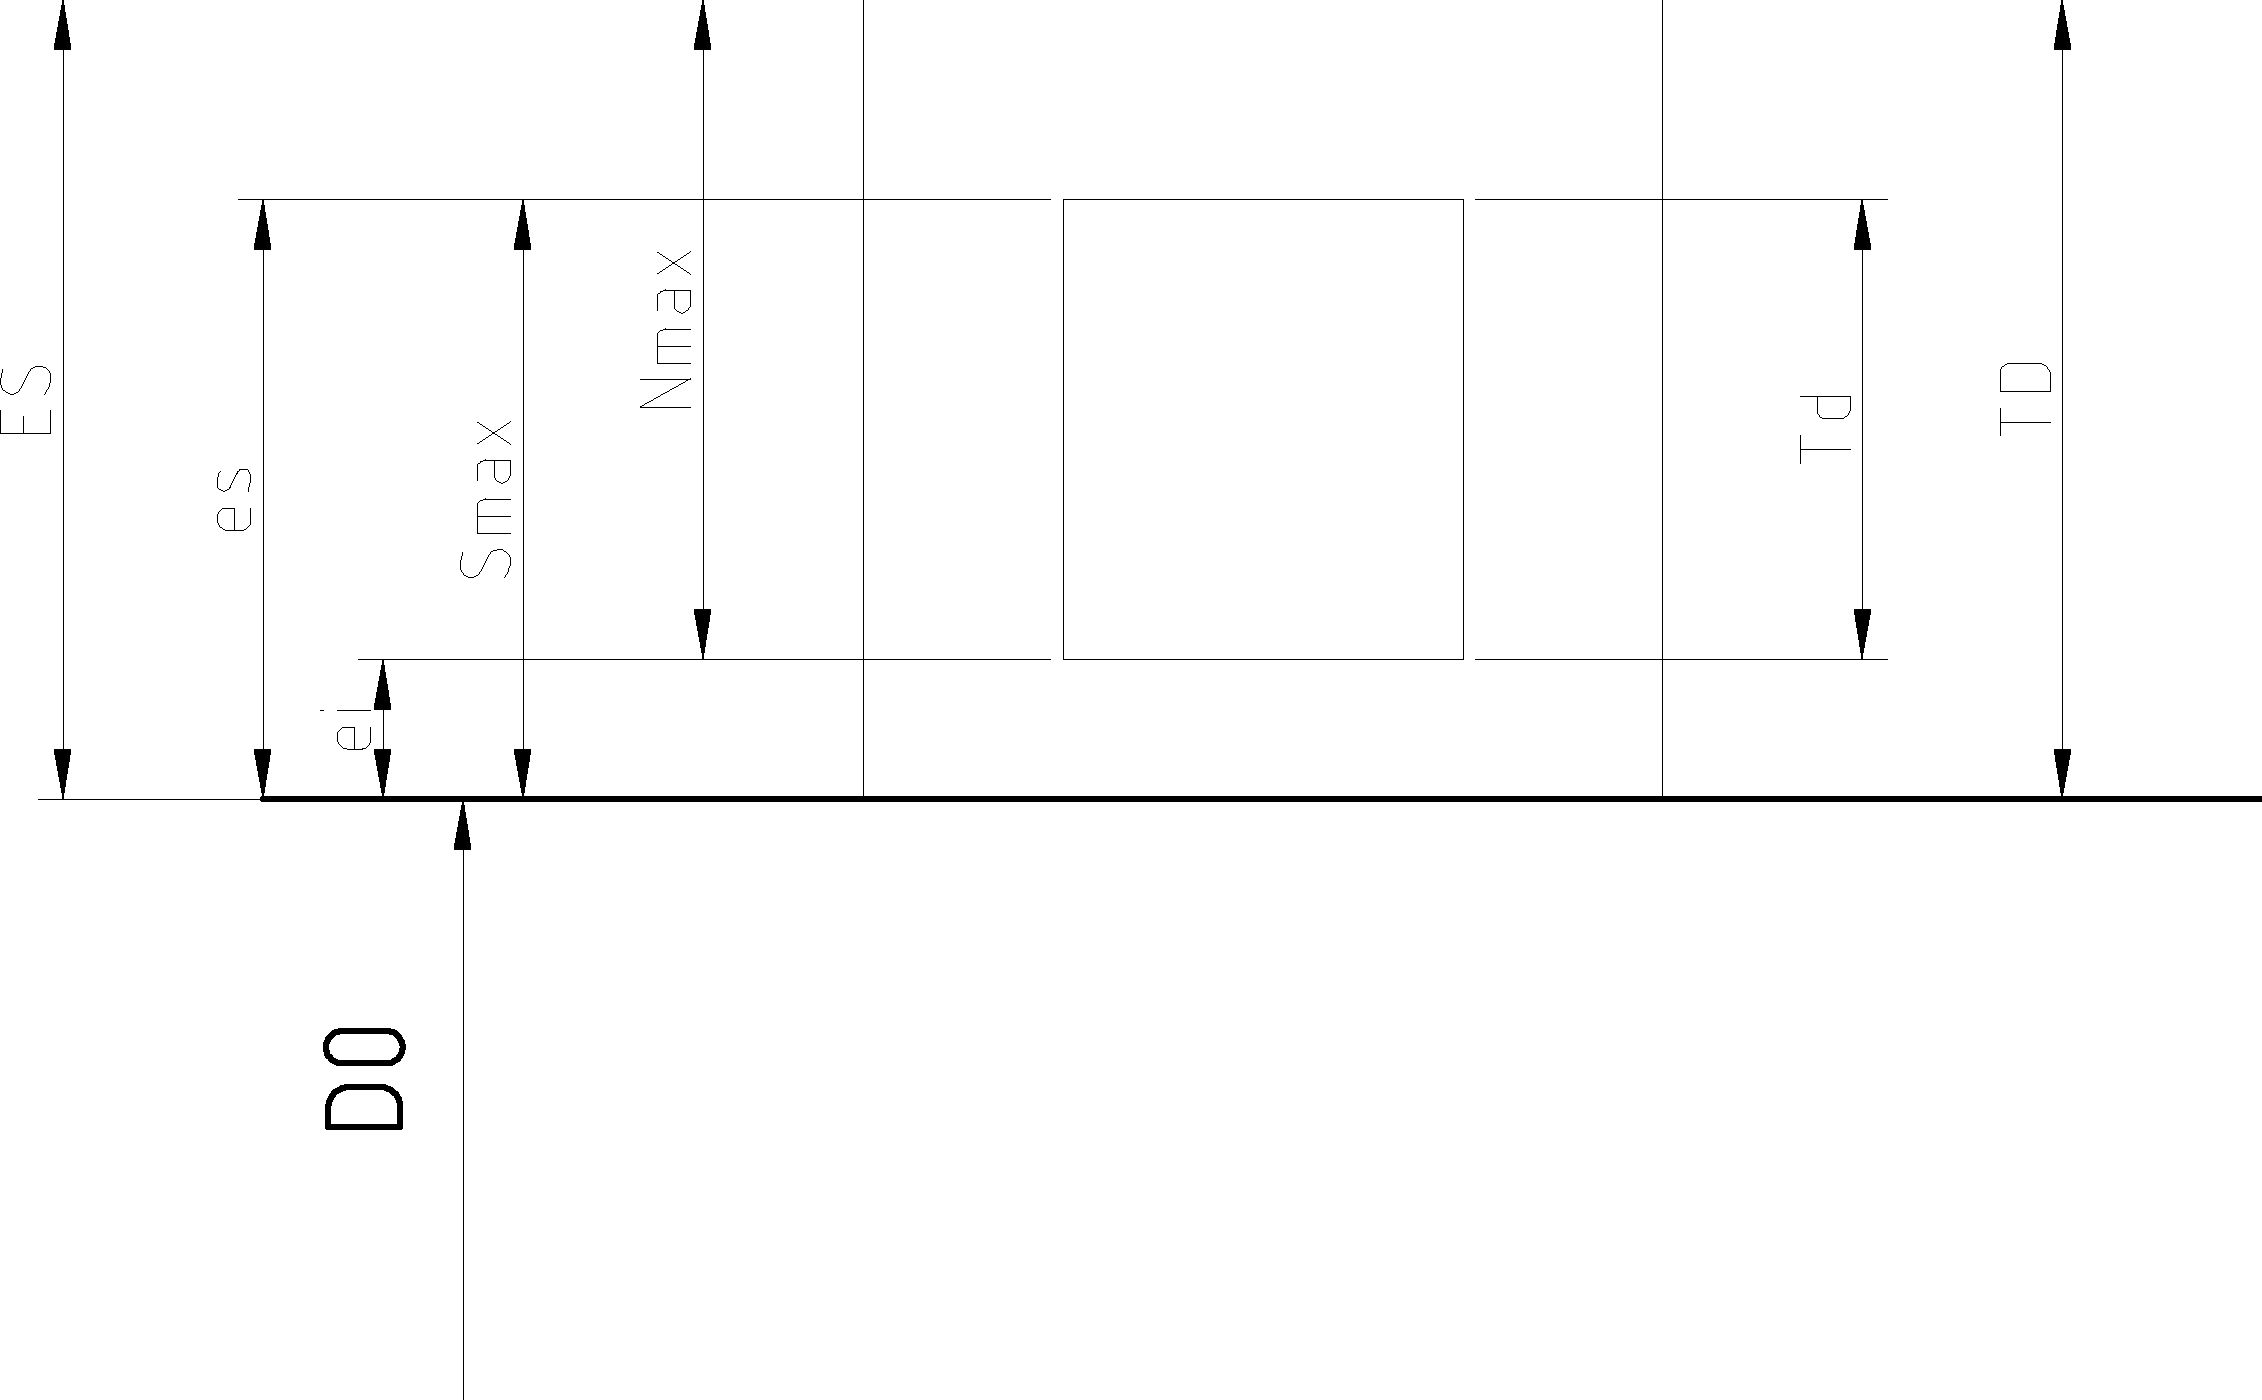
\includegraphics[width=0.7\linewidth]{pic/1_1}
	\caption{Посадка с натягом}
	\label{fig:11}
\end{figure}


\section{Характеристики системы допусков и посадок главных цилиндрических соединений}

\begin{enumerate}
	\item Обеспечение нормального температурного режима: $t_{дет} = t_{изм}$ --- совместная выдержка детали и измерительного средства
	\item Единица допуска --- связывает точность с самим размером (устанавливают экспериментально). $IT = k \cdot i$, $i = 0.45 \sqrt[3]{D} + 0.001D$
	\item Квалитет --- совокупность допусков, характеризуемых постоянной относительной точностью, определяемый коэффициентом $k$, для всех номинальных размеров данного диапазона.
	\item Ряд допусков --- строится на основании единицы допуска и квалитета точности.
	\item Диаметры по интервалам распределены так, чтобы допуски, рассчитанные по крайним значениям диаметров и средним отличалось бы не более, чем на 5-8\%.
\end{enumerate}

\section{Основные отклонения валов и отверстий}

Основным отклонением называется одно из двух предельных, ближе расположенное к нулевой линии.

\begin{figure}
	\centering
	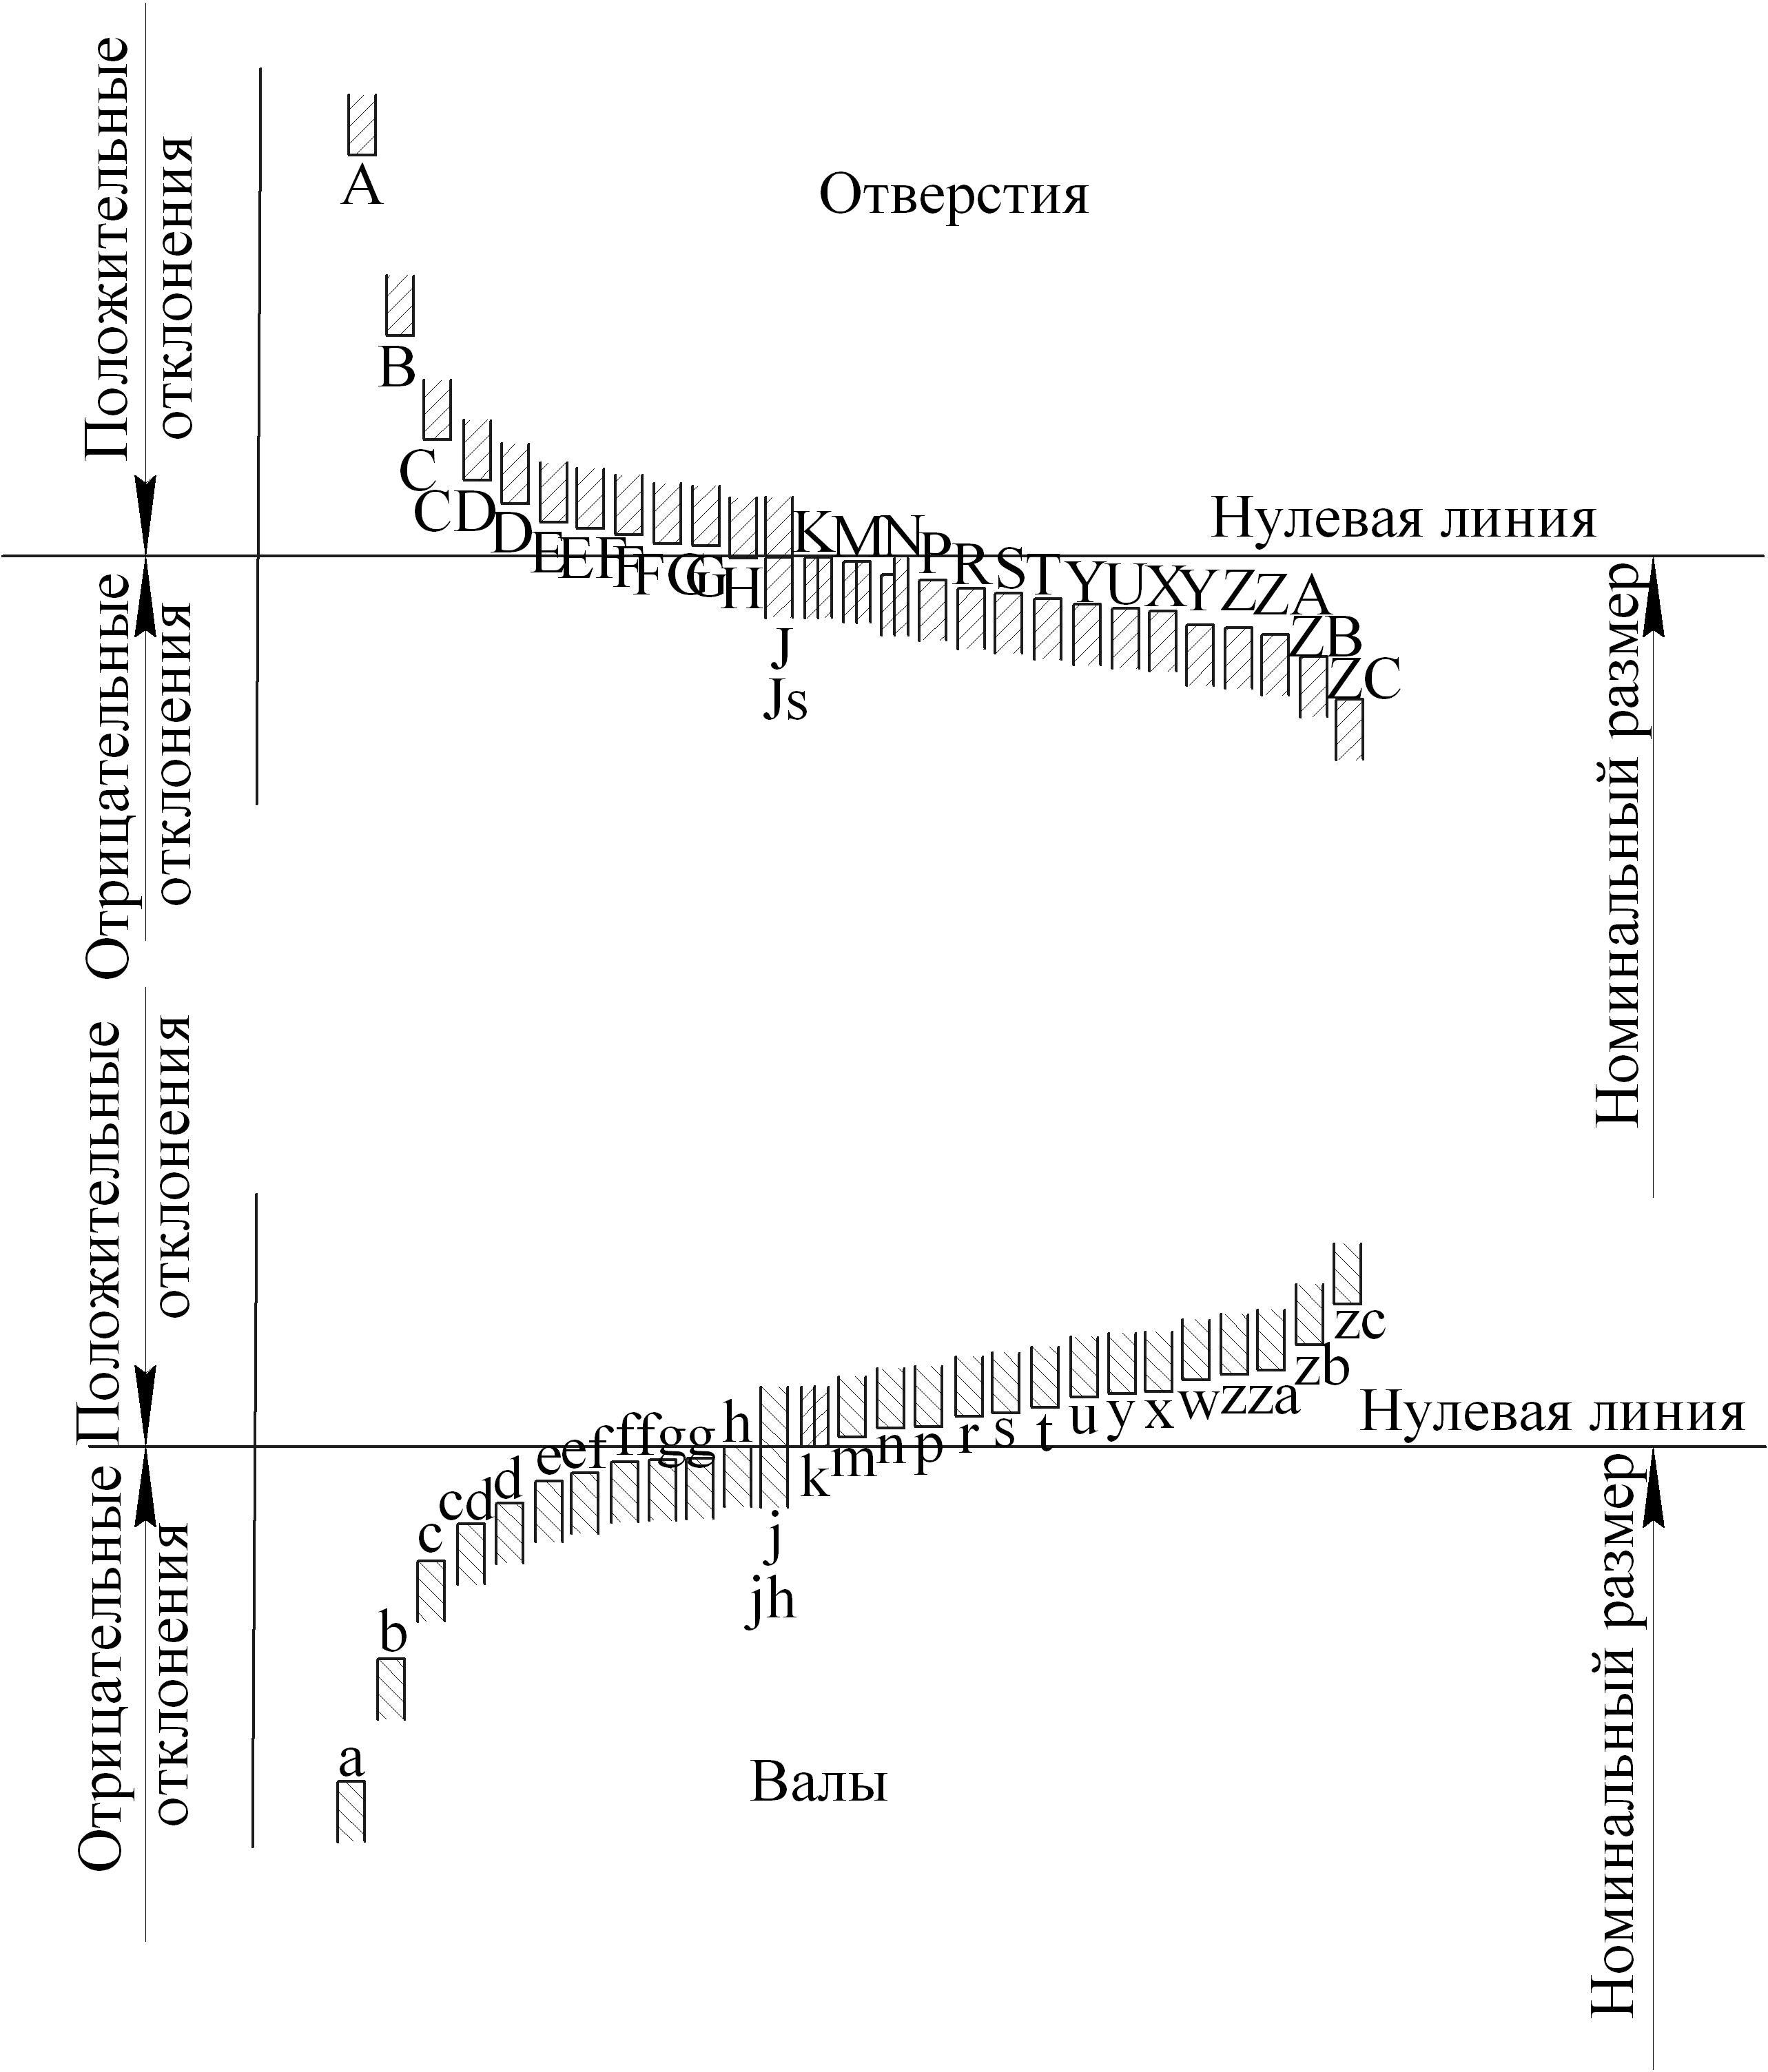
\includegraphics[width=0.7\linewidth]{pic/1_3}
	\caption{Основные отклонения валов и отверстий}
	\label{fig:13}
\end{figure}

 Основные отклонения отверстий построены таким образом, чтобы обеспечить образование посадок в системе вала, аналогичным посадкам в системе отверстия. Основные отклонения отверстий равны по величине и противоположны по знаку основным отклонениям валов, обозначаемым той же буквой. Основные отклонения отверстий определяются по двум правилам.

Общее правило. Основное отклонение отверстия должно быть симметрично относительно нулевой линии основному отклонению вала, обозначаемому той же буквой: EI = – es для A – H; ES = – ei – для J – ZC.

Специальное правило. Две соответствующие друг другу посадки в системе отверстия и в системе вала, в которых отверстие данного квалитета соединяется с валом ближайшего более точного квалитета, должны иметь одинаковые зазоры или натяги (например, H7/p6 и P7/h6).

\section{Три типа посадок}

\begin{enumerate}
	\item Посадка с зазором --- посадка, при которой в соединении, всегда образуется зазор, т.е. наименьший предельный размер отверстия больше наибольшего предельного размера вала или равен ему.
	
	Наименьший зазор ($S_{\min}$) – разность между наименьшим предельным размером отверстия и наибольшим предельным размером вала в посадке с зазором:
	
	$$S_{\min} = D_{\min} – d_{\max} = EI – es$$
	
	Наибольший зазор ($_{S\max}$) – разность между наибольшим предельным размером отверстия и наименьшим предельным размером вала в посадке с зазором или в переходной посадке
	
	$$S_{\max} = D_{\max} – d_{\min} = ES – ei$$
	
	Средний зазор ($S_c$) – это среднее арифметическое наибольшего и наименьшего зазоров.
	
	\item Посадка с натягом - посадка, при которой в соединении всегда образуется натяг, т.е. наибольший предельный размер отверстия меньше наименьшего предельного размера вала или равен ему.
	
	Наименьший натяг ($N_{\min}$) – разность между наименьшим предельным размером вала и наибольшим предельным размером отверстия до сборки в посадке с натягом:.
	
	$$N_{\min} = d_{\min} – D_{\max} = ei – ES$$
	
	Наибольший натяг ($N\max$) – разность между наибольшим предельным размером вала и наименьшим предельным размером отверстия до сборки в посадке с натягом или в переходной посадке:
	
	$$N_{\max} = d_{\max} – D_{\min} = es – EI$$
	
	Средний натяг ($N_c$) – это среднее арифметическое наибольшего и наименьшего натягов
	
	\item 	Переходная посадка - посадка, при которой в соединении возможно получение как зазора, так и натяга, в зависимости от действительных размеров отверстия и вала.
	
	Переходная посадка характеризуется наибольшими значениями натяга ($N_{\max}$) и зазора ($S_{\max}$)
\end{enumerate}

\begin{figure}
	\centering
	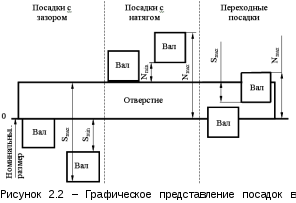
\includegraphics[width=0.7\linewidth]{pic/1_4}
	\caption{Три типа посадок}
	\label{fig:14}
\end{figure}

\section{Посадки в системе отверстия}

Посадки в системе отверстия – посадки, в которых требуемые зазоры и натяги получаются сочетанием различных полей допусков валов с полем допуска основного отверстия, обозначаемого буквой H. Основное отверстие – отверстие, нижнее отклонение которого равно нулю.

\section{Посадки в системе вала}

Посадки в системе вала – посадки, в которых требуемые зазоры и натяги получаются сочетанием различных полей допусков отверстий с полем допуска основного вала, обозначаемого буквой h. Основной вал – вал, верхнее отклонение которого равно нулю.

\section{Посадки с зазором}

Посадки с зазором предназначены для подвижных и неподвижных соединений. Посадки рассчитаны на следующие условия их применения: нормальный температурный режим работы, близкие коэффициенты линейных расширений материалов деталей.

\section{Посадки с натягом}

 Посадки применяются только в точных квалитетах, используются для передачи крутящих моментов и осевых сил без дополнительного крепления.

Посадки предназначены для неподвижных и неразъемных соединений. Относительная неподвижность обеспечивается силами трения, возникающими на контактирующих поверхностях вследствие упругой деформации, создаваемой натягом при сборке соединения.

\section{Переходные посадки}

 Переходные посадки применяются только в точных квалитетах – с 4-го по 8-й и используются как центрирующие посадки. Предназначены для неподвижных, но разъемных соединений, так как обеспечивают легкую сборку и разборку соединения.

Переходные посадки требуют, как правило, дополнительного крепления соединяемых деталей.

\section{Посадки подшипников качения}

В зависимости от условий работы узла или механизма в целом различают местное, циркуляционное и колебательное нагружения колец подшипников. При местном нагружении кольцо неподвижно и нагрузка направлена и действует на одно и то же место в кольце. При циркуля­ционном нагружении за каждый оборот подшипника последовательно нагружаются все участки окружности дорожки качения кольца. При колебательном нагружении лишь определенный участок кольца пооче­редно подвергается нагрузке.

Соединение вращающихся относительно нагрузки колец с валом или корпусом выполняют обязательно с натягом.

Предельные отклонения размеров посадочных поверхностей подшип­ников класса точности 0 регламентированы ГОСТ 520-89 «Подшипники качения. Технические требования». Посадки подшипников отличаются от обычных расположением и величинами полей допусков на поса­дочные поверхности колец.

\section{Отклонение формы поверхностей}

Реальная поверхность --- поверхность, ограничивающая деталь и полученная в результате обработки.

Номинальная поверхность --- идеальная поверхность, номинальная форма которой задана на чертеже.

Действительная поверхность --- поверхность, воспроизведенная по размерам, измеренным с допусками.

Прилегающая поверхность: имеет форму номинальной поверхности; соприкасается с реальной поверхностью; расположена вне материала так, что расстояние до наиболее удаленной точки реальной поверхности минимально (расстояние измеряется по нормали и прилегающей поверхности).

\begin{tabular}{|c|c|}
	\hline 
	Вид допуска формы & Обозначение \\ 
	\hline 
	Допуск прямолинейности & 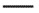
\includegraphics{pic/dop_form/index.jpg}  \\ 
	\hline 
	Допуск плоскостности & 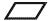
\includegraphics{pic/dop_form/get.jpg}  \\ 
	\hline 
	Допуск круглости & 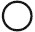
\includegraphics{pic/dop_form/index1.jpg} \\ 
	\hline 
	Допуск цилиндричности & 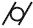
\includegraphics{pic/dop_form/index2.jpg} \\ 
	\hline 
	Допуск профиля продольного сечения & 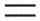
\includegraphics{pic/dop_form/get1.jpg} \\ 
	\hline 
\end{tabular} 

Отклонение от прямолинейности --- область на плоскости, ограниченная двумя параллельными прямыми, расположенными друг от друга на расстоянии, равном допуску прямолинейности Т.

Отклонение плоскостности --- наибольшее расстояние от точек реальной поверхности (профиля) до прилегающей плоскости (прямой) в пределах нормируемого участка

Отклонение от круглости --- наибольшее расстояние от точек реального профиля до прилегающей окружности.

Прилегающая окружность --- окружность минимального диаметра, описанная вокруг реального профиля наружной поверхности вращения, или окружность максимального диаметра, вписанная в реальный профиль внутренней поверхности. 

Отклонение от цилиндричности - наибольшее расстояние от точек реальной поверхности до прилегающего цилиндра в приделах нормируемого участка.

Отклонение от профиля продольного сечения - наибольшее расстояние от точек образованной реальной поверхности и лежащих в плоскости проходящей через ось до соответствующей стороны прилегающего профиля. В приделах нормируемого участка.

\section{Отклонения расположения поверхностей и осей}

\begin{tabular}{|c|c|}
	\hline 
	Допуски расположения & Обозначение \\ 
	\hline 
	Допуск параллельности & 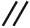
\includegraphics{pic/dop_rasp/index.jpg}  \\ 
	\hline 
	Допуск перпендикулярности & 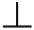
\includegraphics{pic/dop_rasp/index1.jpg} \\ 
	\hline 
	Допуск наклона & 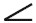
\includegraphics{pic/dop_rasp/index2.jpg} \\ 
	\hline 
	Допуск соосности & 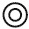
\includegraphics{pic/dop_rasp/index4.jpg} \\ 
	\hline 
	Допуск симметричности & 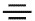
\includegraphics{pic/dop_rasp/index6.jpg} \\ 
	\hline 
	Позиционный допуск & 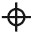
\includegraphics{pic/dop_rasp/index7.jpg} \\ 
	\hline 
	Допуск пересечения осей & 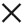
\includegraphics{pic/dop_rasp/index8.jpg} \\ 
	\hline 
\end{tabular} 

Отклонение от параллельности(EPA) --- разность наибольшего и наименьшего расстояний между плоскостями в пределах нормируемого участка.

Отклонение от перпендикулярности плоскостей(EPR) --- отклонение угла между плоскостями от прямого угла, выраженное в линейных единицах на длине нормируемого участка.

Отклонение наклона (EPN):отклонение угла между рассматриваемым элементом (плоскостью, осью) и базой от номинального угла, выраженное в линейных единицах на длине нормируемого участка.

Отклонение от соосности (EPC):наибольшее расстояние между осью рассматриваемой поверхности вращения и базой (осью базовой поверхности или общей осью двух или нескольких поверхностей) на длине нормируемого участка.

Отклонение от симметричности (EPS):наибольшее расстояние между плоскостью симметрии (осью) рассматриваемого элемента (элементов) и базой – плоскостью симметрии базового элемента, осью или общей плоскостью симметрии двух или нескольких элементов в пределах нормируемого участка.

Позиционное отклонение (EPP):наибольшее расстояние между реальным расположением элемента (его центра, оси или плоскости симметрии) и его номинальным расположением в пределах нормируемого участка.

Отклонение от пересечения осей (EPX):наименьшее расстояние между осями, номинально пересекающимися.

